\section{Introduction}
\subsection*{Objective}
The objective of our project was to take a 3 degree of freedom (DOF) robot manipulator and move an object of unknown mass from an initial state to a specified goal state, and then return the manipulator to its original position.
Three primary methods were experimented with in this project.
The first involved developing a method to estimate the mass matrix of the manipulator, with which a controller was designed to track the arm to the initial state, and back home when the object had been dropped in the goal state.
The second part involved using a Kalman filter to estimate the positions of the initial state, goal state, and the current joint configurations of the manipulator.
The last part was developing an adaptive controller to account for the unknown mass of the object to move it successfully from the initial state to the goal state.

\subsubsection*{Ancillary Tasks}
While not the focus of our project, several other components were required in order to complete the described task.
These include the following:

\begin{itemize}
  \item Path planning algorithm (RRT*)
  \item Trajectory planner
  \item Collision detection
  \item Inverse kinematics to map Cartesian space target into joint space
\end{itemize}

\noindent These items are mentioned here for completeness sake, but are not discussed in details in the report as they were not the primary objective.

\section{Robotic Modeling}
\subsection{Approach}

The general equation of motion for a robotic manipulator can be expressed as:

\begin{equation}
  \label{eom-manipulator}
  M(q)\ddot{q} + C(q,\dot{q})\dot{q} + G(g) = \tau
\end{equation}

\noindent where $M(q)\in\mathbb{R}^{n\times n}$ is the mass matrix of the joints,
$C(q,\dot{q})\in\mathbb{R}^{n\times n}$ is the Coriolis matrix,
$G(q)\in\mathbb{R}^{n}$ is the conservative force vector acted on the arm by
gravity, and $\tau\in\mathbb{R}^{n}$ are the torques commanded to each joint.
Each of the terms on the left hand side of the equation can be directly modeled
when the manipulator joint information is known.
However, when this information is not available, a neural network can be used to
estimate the value of these matrices.

To model the conservative force vector, a robotic manipulator can be controlled
with a simple PD controller and brought to a stop at a given configuration value
$q$.
When the manipulator is at rest, Eq. (\ref{eom-manipulator}) simplifies to:

\begin{align}
  \label{eom-manipulator-stopped}
  M(q)*0 + C(q,0)*0 + G(q) &= \tau\\
  G(q) &= \tau
\end{align}

\noindent which allows the loss function for the function approximator
$\hat{G}(q)$ to be expressed as:

\begin{equation}
  \label{loss-function-gq}
  \hat{G}(q) - \tau = \delta_{Loss}
\end{equation}

To model the mass matrix with a function approximator $\hat{M}(q)$, we must
again model a loss function to train the network.
This proves more difficult, as the mass matrix must be isolated on the left hand
side of the equation.
However, if the number of acceleration samples taken at a given configuration
$q$ satisfy $rk(M(q)) = n_{samples}$, we could then construct an acceleration
matrix $\ddot{Q} = [\ddot{q_{1}}, \ddot{q_{2}}\dots\ddot{q_{n}}]$ which
satisfies $rk(\ddot{Q}) = rk(M(q)) = n$.
Properties of linear algebra now guarantee that a unique inverse of this matrix
must exist, and the equation can then be expressed as:

\begin{align}
  \label{eom-manipulator-accel}
  M(q)\ddot{Q} + C(q,\dot{Q})\dot{Q} + G(q) &= \tau\\
  \label{eom-manipulator-accel-m}
  M(q) &= \ddot{Q}^{-1}(\tau - G(q) - C(q,\dot{Q})\dot{Q})
\end{align}

The problem with this method is that the Coriolis term is still in place, and we
have no estimate for this value.
However, if we take our $\ddot{q}$ samples at the initial point when we first
begin accelerating, we should see that $\dot{q} \approx 0$, and thus Eq.
(\ref{eom-manipulator-accel-m}) can be expressed as:

\begin{align}
  M(q) = \ddot{Q}^{-1}(\tau - G(q))
\end{align}

\noindent which now allows for a loss function to be formulated.

For the Coriolis matrix, it directly depends on the mass matrix $M(q)$, and thus
once an estimate for $M(q)$ is formulated, the Coriolis matrix can be derived
from the given values of the $\hat{M}(q)$ matrix.

\subsection{Experiments}
The experiments for this section will include learning both $\hat{G}(q)$ and
$\hat{M}(q)$ using the proposed method above in two settings: One in a friction
free environment, and another when static friction is present.
The friction free case will be used primarily as a base case, and the accuracy
of both the $\hat{G}(q)$ and $\hat{M}(q)$ will be compared to their true values.
This will serve to see how effective this method is in general, as
friction begins complicating the process.

The frictional case will be further broken down into two sections.
The first will consist of learning the two maps without static friction
compensation, and the second will include static friction compensation.
Static friction will be modeled as a constant $\mu_{s}$, so this can easily be
added into the above formulations (primarily for the mass matrix case).

\section{Perception and Planning}
\subsection{Uncertainty in Configurations and Perception}
At the end-effector of our robot there is a camera.  This camera will be able to perceive the obstacles and the movable object in the space.  How the camera generates this data is not a concern of this project, so all the measurements being taken are implied to be from the camera.  The camera will sense where the objects are, and thus generate a collision free path to that object.  The error in the position of the end-effector can be a result of multiple sources: uncertainty in the camera's measurements and uncertainty in the joint configurations.  A Kalman Filter will be implemented into our robot to help take care of the noise present in the system.  As the Kalman Filter proceeds, the state becomes closer to the true state.  While the Kalman filter works, the outputs will be fed into the controls of the robot to generate the desired behavior.
\subsection*{Control Models}
To validate our control models, it is important to evaluate the error dynamics associated with the controllers. To do this, we begin with the comparison of the error convergence between the Adaptive Control model and the classical PD Control model. This comparison was made with a fixed, known weight, as well as no noise in the joint values.
\begin{figure}[H]
	\centering
	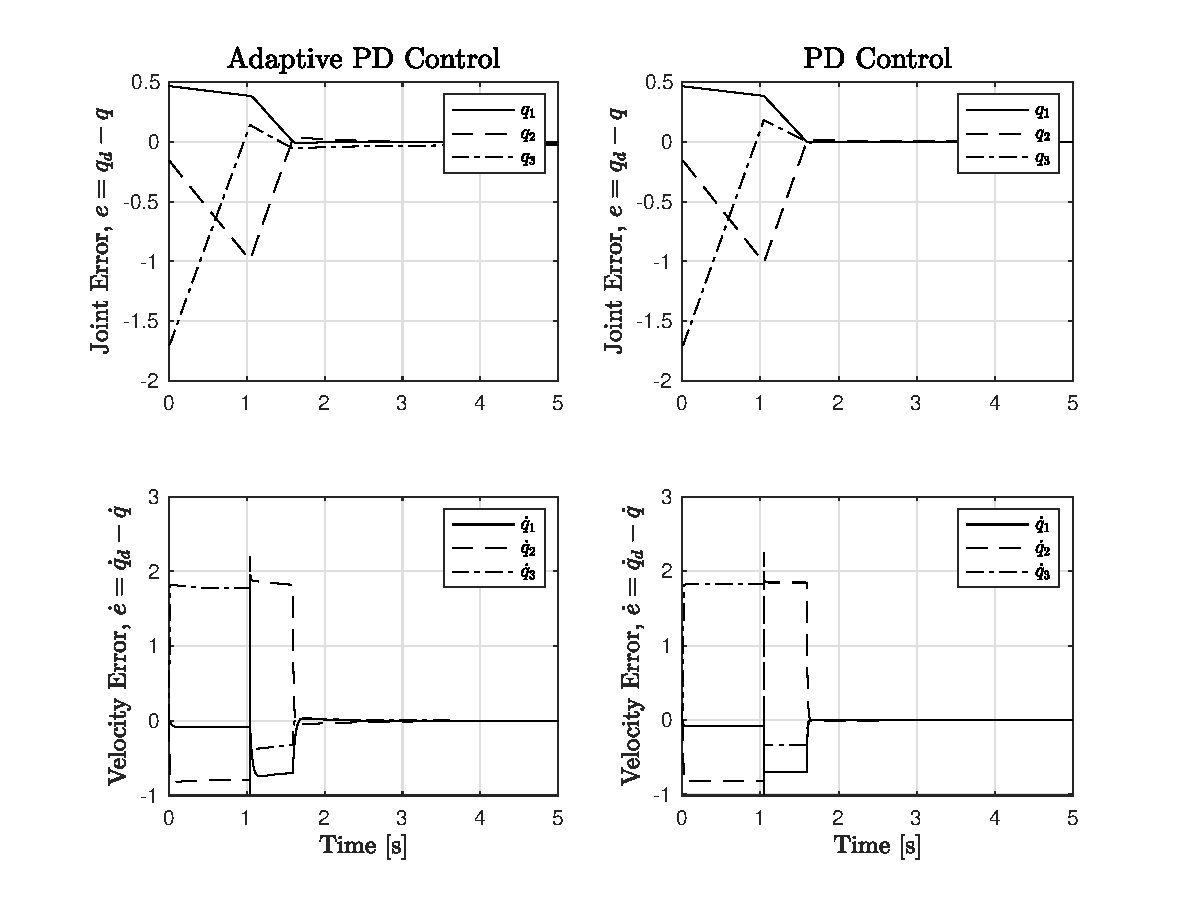
\includegraphics[width=0.7\textwidth]{figures/adpdErr.eps}
	\caption{Convergence of controller error dynamics}
	\label{fig:adpderr}
\end{figure}
As shown in Fig. \ref{fig:adpderr}, both controllers converge to the steady state value of zero in approximately the same time. One benefit to adaptive control however, is that as the mass changes (i.e. an object is picked up), the adaptation law accounts for the change in mass. With PD Control, there is no way to account for this mass addition and an increase in error is introduced.\\

We then evaluate each controller by it's ability to follow the desired trajectory provided by the $RRT^{*}$ path planning algorithm.
\begin{figure}[H]
	\centering
	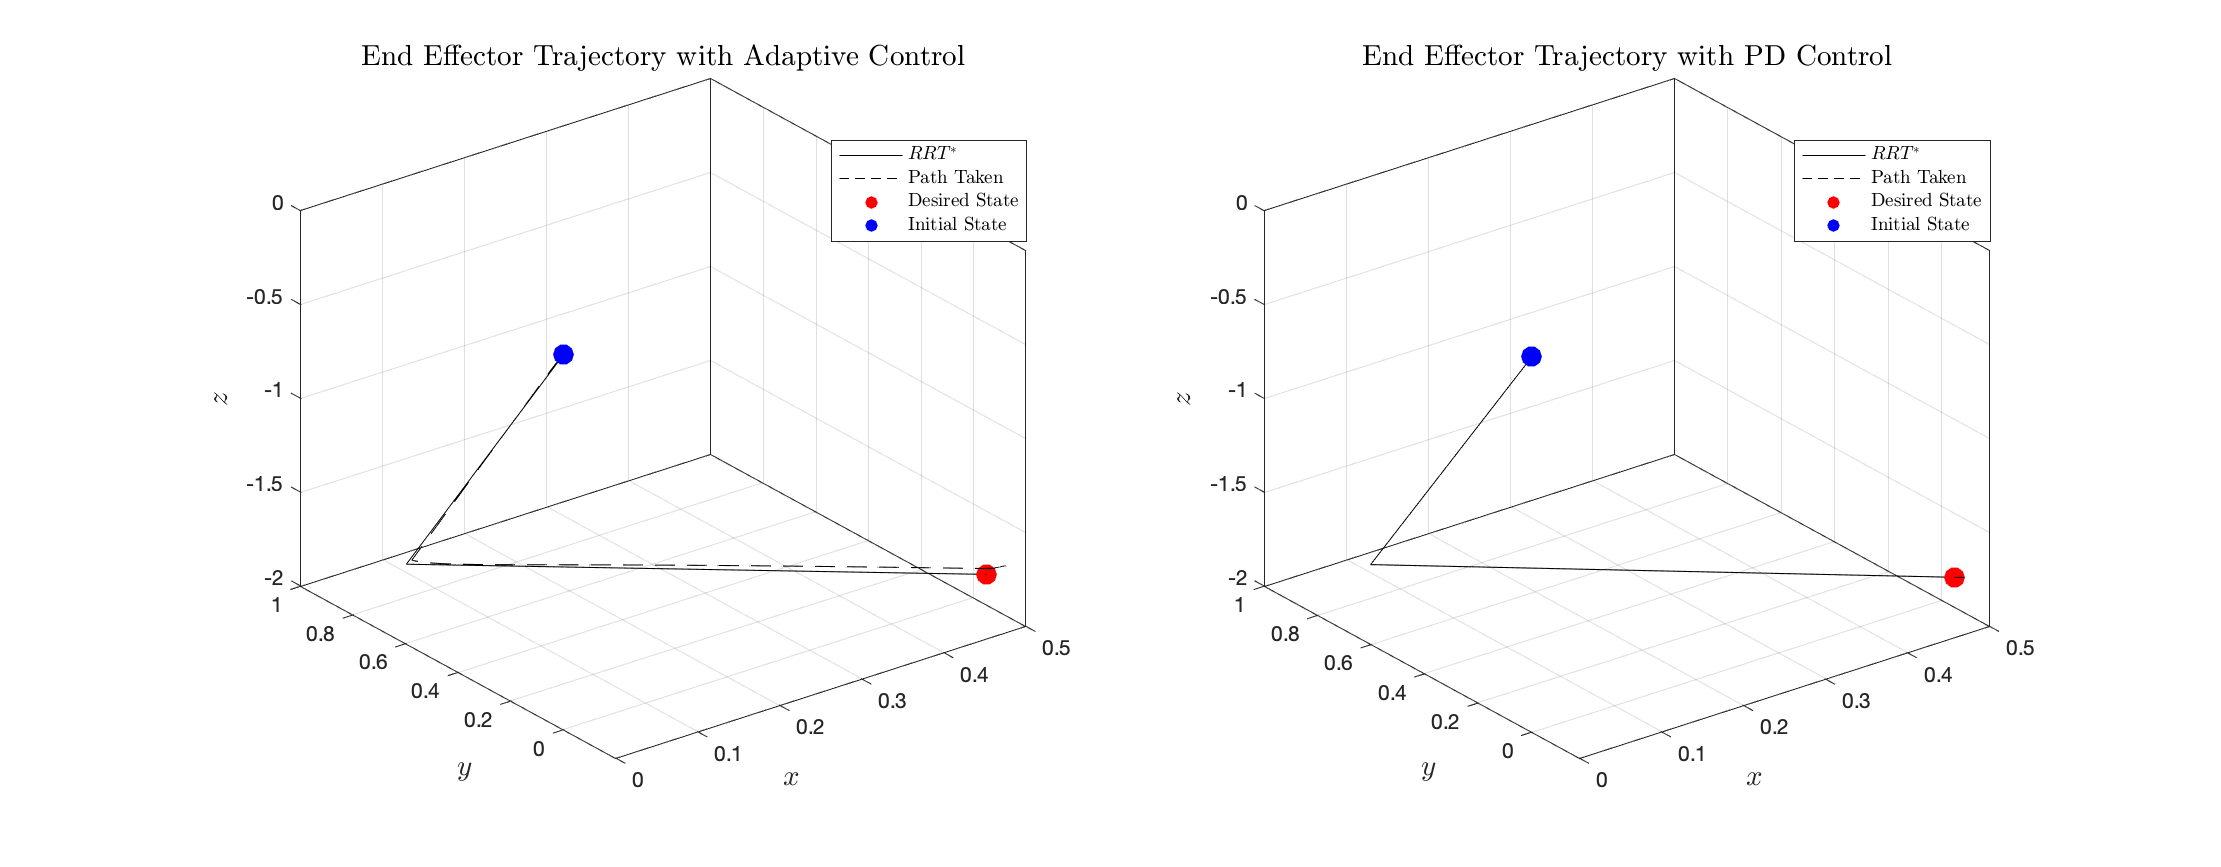
\includegraphics[width=0.9\textwidth]{figures/eeTraj.eps}
	\caption{Desired end-effector trajectory vs actual}
	\label{fig:eetraj}
\end{figure}
We can see from Fig. \ref{fig:eetraj} that in this case, the PD Controller maintains the desired trajectory more tightly than the Adaptive Control model. However, the error between the two control models is of an insignificant degree, thus the adaptive control model is chosen for the simulation.

